\documentclass[letterpaper]{article}
\usepackage[margin=1in]{geometry}
\usepackage[utf8]{inputenc}
\usepackage{textcomp}
\usepackage{amssymb}
\usepackage{natbib}
\usepackage{graphicx}
\usepackage{gensymb}
\usepackage{amsthm, amsmath, mathtools}
\usepackage[dvipsnames]{xcolor}
\usepackage{enumerate}
\usepackage{mdframed}
\usepackage[most]{tcolorbox}
\usepackage{csquotes}
% https://tex.stackexchange.com/questions/13506/how-to-continue-the-framed-text-box-on-multiple-pages

\tcbuselibrary{theorems}

\newcommand{\R}{\mathbb{R}}
\newcommand{\Z}{\mathbb{Z}}
\newcommand{\N}{\mathbb{N}}
\newcommand{\Q}{\mathbb{Q}}
\newcommand{\C}{\mathbb{C}}
\newcommand{\code}[1]{\texttt{#1}}
\newcommand{\mdiamond}{$\diamondsuit$}
\newcommand{\PowerSet}{\mathcal{P}}
\newcommand{\Mod}[1]{\ (\mathrm{mod}\ #1)}
\DeclareMathOperator{\lcm}{lcm}

%\newtheorem*{theorem}{Theorem}
%\newtheorem*{definition}{Definition}
%\newtheorem*{corollary}{Corollary}
%\newtheorem*{lemma}{Lemma}
\newtheorem*{proposition}{Proposition}


\newtcbtheorem[number within=section]{theorem}{Theorem}
{colback=green!5,colframe=green!35!black,fonttitle=\bfseries}{th}

\newtcbtheorem[number within=section]{definition}{Definition}
{colback=blue!5,colframe=blue!35!black,fonttitle=\bfseries}{def}

\newtcbtheorem[number within=section]{corollary}{Corollary}
{colback=yellow!5,colframe=yellow!35!black,fonttitle=\bfseries}{cor}

\newtcbtheorem[number within=section]{lemma}{Lemma}
{colback=red!5,colframe=red!35!black,fonttitle=\bfseries}{lem}

\newtcbtheorem[number within=section]{example}{Example}
{colback=white!5,colframe=white!35!black,fonttitle=\bfseries}{def}

\newtcbtheorem[number within=section]{note}{Important Note}{
        enhanced,
        sharp corners,
        attach boxed title to top left={
            xshift=-1mm,
            yshift=-5mm,
            yshifttext=-1mm
        },
        top=1.5em,
        colback=white,
        colframe=black,
        fonttitle=\bfseries,
        boxed title style={
            sharp corners,
            size=small,
            colback=red!75!black,
            colframe=red!75!black,
        } 
    }{impnote}
\usepackage[utf8]{inputenc}
\usepackage[english]{babel}
\usepackage{fancyhdr}
\usepackage[hidelinks]{hyperref}

\pagestyle{fancy}
\fancyhf{}
\rhead{CSE 101}
\chead{Monday, February 14, 2022}
\lhead{Lecture 16}
\rfoot{\thepage}

\setlength{\parindent}{0pt}

\begin{document}

\section{Greedy Algorithm}
We continue our discussion of greedy algorithms.

\subsection{Problem: Minimum Spanning Trees}
Given a weighted graph $G$, find a minimum spanning tree of $G$. 

\subsubsection{Tree}
\begin{definition}{}{}
    A \textbf{tree} is a connected, \emph{undirected} graph with no cycles. 
\end{definition}
\textbf{Remark:} This is different from a DAG. 

\subsubsection{Spanning Tree}
\begin{definition}{}{}
    A \textbf{spanning tree} for a graph $G$ is a subset $T$ of the \emph{edges} of $G$ such that
    \begin{itemize}
        \item The edges forms a tree. 
        \item All vertices in $G$ are covered in $T$; that is, the vertices in $T$ are the same as the vertices in $G$. 
    \end{itemize}
\end{definition}

\subsubsection{Minimum Spanning Tree}
\begin{definition}{}{}
    Given a weighted graph $G$, a \textbf{minimum spanning tree} of $G$ is a spanning tree where the sum of the weights of the edges are as small as possible. 
\end{definition}

\subsubsection{Tree Properties}
\begin{lemma}{}{}
    For an undirected graph $G = (V, E)$, any two of the below imply the third. 
    \begin{enumerate}
        \item $|E| = |V| - 1$. 
        \item $G$ is connected. 
        \item $G$ has no cycles. 
    \end{enumerate}
\end{lemma}

\begin{mdframed}[]
    \begin{proof}
        Suppose we build $G$ one edge at a time. Initially, we have $|V|$ many connected components with 0 edges. When we add an edge, this reduces the number of connected components by one unless the new edge is part of a cycle. To show this, suppose we have connected components $A$, $B$, $C$, and $D$. 
        \begin{itemize}
            \item \underline{Case 1: Not Cycles.} Suppose we have an edge connecting $A$ to $B$. Since this edge is not part of a cycle, there are now three connected components.
            \item \underline{Case 2: Cycles.} Suppose $A$ has two vertices $A'$ and $A''$, and we connect an edge from $A'$ to $A''$. Since $A'$ and $A''$ are in this connected component $A$, this implies that there was already a edge from $A'$ to $A''$. Therefore, adding another edge creates a cycle. Clearly, this doesn't reduce the number of connected components. 
        \end{itemize}
        If there are no cycles, then it will be the case that the number of connected components will be $|V| - |E|$. On the other hand, if there are cycles, the number of connected components will be bigger than $|V| - |E|$. From this alone, we can show that the lemma holds for two of the conditions. 
        \begin{itemize}
            \item If we assume that (1) and (2) holds, then since $G$ is connected, the number of connected components is 1. On the other hands, $|V| - |E|$ is also equal to 1, so there must be no cycles. 
            \item If we assume that (1) and (3) holds, then since $G$ has no cycles, then $|V| - |E| = 1$, so there is one connected component, and thus the graph is connected.
            \item If we assume that (2) and (3) holds, then again we know that the number of connected components is 1 since we're connected, so the number of edges must be one less than the number of vertices.
        \end{itemize}
        This proves the lemma. 
    \end{proof}
\end{mdframed}

\begin{corollary}{}{}
    If $G$ is a tree, then $|E| = |V| - 1$. 
\end{corollary}

\subsubsection{Intuition for a Greedy Algorithm}
The intuitive -- and obvious -- way to begin is to just pick the edge with the smallest weight. That edge will be a part of your tree. From there, it becomes somewhat unclear what we should do. However, this works! 

\begin{lemma}{}{}
    If $e$ is a minimum weight edge in $G$, then there is a minimum spanning tree of $G$ that contains $e$. 

    \bigskip 

    If $e$ is a unique minimum weight edge in $G$, then all minimum spanning trees of $G$ will contain $e$. 
\end{lemma}

\begin{mdframed}[]
    \begin{proof}
        Take a minimum spanning tree $T$. If $e \in T$, then we're done. Otherwise, suppose we add $e$ to our minimum spanning tree. Then, we get a cycle. So, we can find some other $e'$ in this cycle and let $T' = T \cup \{e\} \setminus \{e'\}$. This is another spanning tree as the tree is still connected with the right number of edges. Then, the weight of $T'$ is given by 
        \[w(T') = w(T) + w(e) - w(e')\]
        but since $e$ is a minimum weight edge, and the weight of $e$ must be no more than $e'$, so it follows that 
        \[w(T') \leq w(T)\] 
        Additionally, if $e$ is a unique minimum weight edge, then $w(T') < w(T)$. So, we are done. 
    \end{proof}
\end{mdframed}

\subsubsection{Example: MST}
\begin{center}
    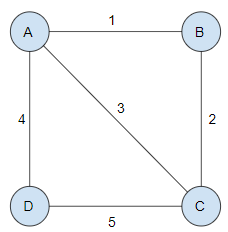
\includegraphics[scale=0.6]{../assets/mst_1.png}
\end{center}
Consider the graph above. Find the minimum spanning tree. 

\begin{mdframed}[]
    From our lemma, we know that the edge of weight 1 must be in the tree since it is minimal. So, we can select it. 
    \begin{center}
        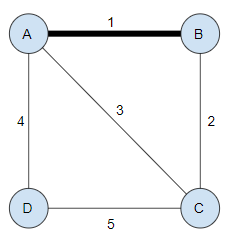
\includegraphics[scale=0.8]{../assets/mst_2.png}
    \end{center}
    Our lemma doesn't say anything about what to do when we have to consider multiple edges. However, we can use a trick -- something we know is that $A$ and $B$ essentially form a connected component, so we can ``merge'' them together.
    \begin{center}
        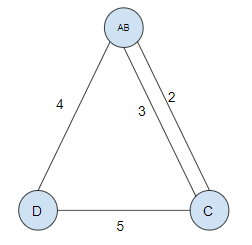
\includegraphics[scale=0.8]{../assets/mst_2a.png}
    \end{center}
    From here, we can see that the edge of weight 2 must be in the tree since it is minimal. So, we can select it. 
    \begin{center}
        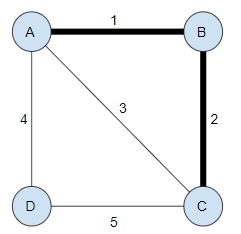
\includegraphics[scale=0.8]{../assets/mst_3.png}
    \end{center}
    Making use of the same trick that we described above, we have: 
    \begin{center}
        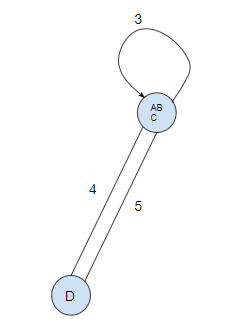
\includegraphics[scale=0.8]{../assets/mst_3a.png}
    \end{center}
    Since MSTs cannot include loops, the edge of weight 4 must be in the tree since it is minimal. So, we can select it.
    \begin{center}
        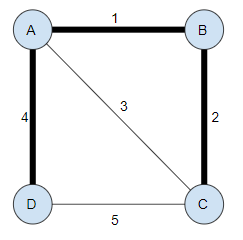
\includegraphics[scale=0.8]{../assets/mst_4.png}
    \end{center}
    Since we have reached every vertex in $G$, we are done. Indeed, if we try to use the trick that we described above, we get: 
    \begin{center}
        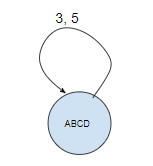
\includegraphics[scale=0.8]{../assets/mst_4a.png}
    \end{center}
    Here, it's obvious that the only edges we need to consider would just loop back, and since we don't allow loops, we are done. 
\end{mdframed}
So, the lemma only gave us the first step of the process. However, by contracting along the edge, we get a new version of the original problem, from which we can apply the lemma again. By repeating this process, we get the MST. 

\subsubsection{Kruskal's Algorithm}
Kruskal's algorithm essentially says to repeatedly add the lightest edge that does not create a cycle. That is: 

\begin{verbatim}
    Kruskal(G):
        T = {}
        while |T| < |V| - 1:
            find lightest e such that T u {e} does not have a cycle 
            add e to T 

        return T 
\end{verbatim}
To check that $T \cup \{e\}$ doesn't create a cycle, we can check if the endpoints of $e$ are in different connected components of $T$. What we mean by this is, if we're just adding the lightest edge every time, it's possible that we'll have several trees; for the sake of simplicity, call these two trees $T_1$ and $T_2$. Then, if one endpoint of an edge $e$ is in $T_1$ and the other endpoint is in $T_2$, then it's not a cycle. If both endpoints $e$ are in $T_1$ or $T_2$ (but not both), then this will form a cycle and so we don't consider this $e$.

\bigskip 

The while loop runs in roughly $\BigO(|V|)$ time. For each iteration, we need to check if there is a cycle that can be formed by picking some $e$; this takes $\BigO(|V|)$ time. Going through all of the edges take $\BigO(|E|)$ time. Therefore, the final runtime is $\BigO(|V|^2 |E|)$ time. 

\subsubsection{First Optimization of Krustal's Algorithm: Recomputing Edge Weights}
Something to note is that, when we're checking edge weights, we're constantly going to see the same edges. If we, for example, add an edge $e = 5$ to our tree, then we don't need to consider the edges with weight less than 5. So, one optimization we can make is to simply not consider any edges that have weight less than the heaviest edge in the tree. So: 
\begin{verbatim}
    Kruskal(G):
        T = {}
        for e in E in increasing order of weight:
            if endpoints in different connected components:
                add e to T 
        return T 
\end{verbatim}
Sorting takes $\BigO(|E|\log(|E|))$. The loop goes through $|E|$ iterations, and computing the connected components takes $|V|$ time. So, our new runtime is 
\[\BigO(|E|\log(|E|) + |V||E|) = \BigO(|V||E|)\]
which is somewhat better. 

\subsubsection{First Optimization of Krustal's Algorithm: Union-Find}
Something else to note is that, when checking connected components, we're essentially computing the same connected components over and over again, all while barely making changes to said connected components. So, we want a data structure that can keep track of a bunch of sets. The idea is that we want a data structure that can
\begin{itemize}
    \item Create a new set: \code{v}
    \item Join two sets: \code{join(v, e)}
    \item Check representative element to see if $v$ and $w$ are in the same set: \code{rep(v)}
\end{itemize}
This is known as the \emph{union-find} data structure. Each set is a directed tree with the representative element at the root. This might look something like\footnote{Imagine each branch pointing upwards, and that each node can have more than 2 children (i.e. it's not a binary tree).}
\begin{verbatim}
                A
               / \ 
              /   \ 
             B     C 
            /|\     \ 
           / | \     \ 
          D  E  F     G 
\end{verbatim}
where the representative is $A$. So, creating a new set takes $\BigO(1)$ time. Finding the representative takes $\BigO(\text{depth of tree})$. Joining two trees (which is as simple as having one representative point to the other representative) takes $\BigO(\text{depth of tree})$ time, since we need to find the representative of the given elements. If we maintain the depth correctly, then the runtimes become $\BigO(\log(\text{number of nodes}))$. 

\bigskip 

So, with this in mind, our revised algorithm is as follows: 
\begin{verbatim}
    Kruskal(G):
        T = {}
        add each v to Union-Find data structure
        for e = (u, v) in increasing order of weight:
            if rep(u) != rep(v):
                add e to T 
                join(u, v)
        return T 
\end{verbatim}
Sorting takes $\BigO(|E|\log(|E|))$. Adding $|V|$ vertices take $\BigO(|V|)$ times ($|V|$ \code{join} calls). Then, iterating through each edge takes $\BigO(|E|)$ time. For each edge, we need to perform $|E|$ \code{rep} operations, and it we have $|V|$ \code{join} operations. Overall, this takes $\BigO(|E|\log(|E|))$ time, assuming we have a reasonable union-find implementation\footnote{Note that the above discussion of union-find is far from ideal. We can make use of, say, path compression to make this more ideal.}. 

\end{document}